\subsection{Does a stronger ordering loss rescue the latent vector?}
The second phase completed 30 new fits: weights 10 and 100, each crossed
with genuine, condition-only, and shuffled heads, for five seeds. Original
AR and $D=2$ references were reevaluated on the same new diagnostic streams.
The raw union contains 26,110 orbits; 25,675 were new and eligible after
excluding the shared history. Each teacher evaluated all eligible structures
afresh. This comparison has its own novelty history and should be read
within its table.

\begin{table}[htbp]
\centering\small
\caption{Primary balanced novel correct-bin yield, percent, mean $\pm$ sample SD over five fit/proposal seeds. Compare arms within this phase's fresh development history.}
\begin{tabular}{lrr}\toprule
Model & UMA & MACE\\\midrule
AR & $61.75\pm2.32$ & $63.19\pm2.01$\\
CVAE $D=2$ / condition controls & $61.04\pm3.72$ & $62.20\pm3.74$\\
Genuine head, $\lambda=10$ & $61.41\pm3.87$ & $62.36\pm3.57$\\
Shuffled target, $\lambda=10$ & $60.59\pm3.26$ & $61.60\pm2.99$\\
Genuine head, $\lambda=100$ & $61.79\pm4.02$ & $63.00\pm3.22$\\
Shuffled target, $\lambda=100$ & $62.26\pm3.59$ & $63.16\pm3.32$\\
\bottomrule\end{tabular}
\end{table}


On sampled posterior latents, the genuine head's mean VAL MSE is
$1.020409\pm0.000255$ for $\lambda=10$ and
$1.020514\pm0.000433$ for $\lambda=100$, with spread over five fits.
Mean KL rises to about 0.0312 nats/mask at $\lambda=100$, but stronger KL is
not accompanied by useful prediction or ordering control. The measured
upper-minus-lower guided change in generated pair fraction is approximately
$-10^{-6}$ and $-3.1\times10^{-5}$, respectively, even having the wrong
average sign for the requested direction.

There is one small positive sampling contrast worth preserving. On UMA,
genuine $\lambda=100$ exceeds its condition-only control by 0.746 percentage
points, with an exploratory paired 95\% interval half-width of 0.658 points.
It differs from AR by only 0.035 points and from the shuffled-target model
by $-0.469$ points. This does not identify physical information as the cause
of the gain. The ordering tests, AR comparator, and shuffled comparator are
needed to avoid that inference.

A separate 512-row TRAIN gradient audit verifies manual edge products,
target scaling, and shuffled assignments for all 45 auxiliary models from
the first two phases. Mean genuine auxiliary encoder-gradient norms increase
from approximately 0.00104 to 0.0100 to 0.1348 as $\lambda$ increases from 1
to 10 to 100; the condition-only path is exactly zero. These unweighted
diagnostic norms are not the actual weighted training update or a
convergence criterion. They establish that the target reaches the encoder
and that its strength changes; a disconnected-loss explanation is therefore
insufficient. All ten stronger condition-only controls also reproduce their
ordinary $D=2$ generator tensors and raw proposals exactly.

\subsection{Posterior-mean supervision and a more informative latent diagnosis}
The posterior-mean objective completed all 15 new fits and the 40 matched
diagnostic evaluations, including sampled-head and AR/$D=2$ references.
There were 24,586 raw unique orbits and 24,568 eligible new orbits, evaluated
by both teachers. On this fresh pool, mean-supervised yield is
$63.33\pm1.76$\% under UMA, compared with $63.47\pm0.86$\% for AR and
$63.40\pm2.05$\% for sampled-head supervision. The paired mean-minus-AR
difference is $-0.139$ percentage points, with 95\% interval half-width
1.874 points. MACE gives $64.08\pm1.85$\% for mean supervision and
$64.20\pm1.19$\% for AR. The actual guided upper-minus-lower pair-fraction
response is $(-9.65\pm23.1)\times10^{-6}$ over five fits, again having no
useful directed effect. Its auxiliary gradient reaches the encoder through
$\mu$ without a direct path through $\log\sigma^2$; shared encoder parameters,
reconstruction, and KL can still change the variance. The negative result
is not explained by a missing gradient.

An important distinction emerges from a posthoc diagnostic. The original
ridge probe standardized $\mu$ across mixed-condition data and used a common
latent slope. Large differences between conditions can obscure tiny,
condition-specific structure signals. We therefore fit an additional ridge
probe separately within each condition, scaling each latent coordinate using
TRAIN moments from that cell. The ridge strength stays at one, without
tuning; VAL targets remain held out. Balanced VAL MSE across nine cells is
$0.1009\pm0.0963$ for ordinary $D=2$, $0.0991\pm0.0644$ for sampled-head
supervision, and $0.0759\pm0.0823$ for mean supervision, versus 1.0212 for
the TRAIN-zero reference and approximately 1.025 for shuffled-target probes.
Thus the deterministic mean retains a recoverable ordering fingerprint.

This fingerprint is not necessarily learned. In the fixed 24-Li, MIDDLE-bin
cell, five random-initialized graph encoders give probe MSE
$0.00671\pm0.00591$, compared with $0.0809\pm0.0567$ for trained $D=2$.
Nonlinear message passing and pooling already encode pair correlations
through the supplied physical graph. These random-feature controls prevent
interpreting a colored latent scatter as evidence that training discovered a
useful physical coordinate.

\begin{figure}[htbp]
\centering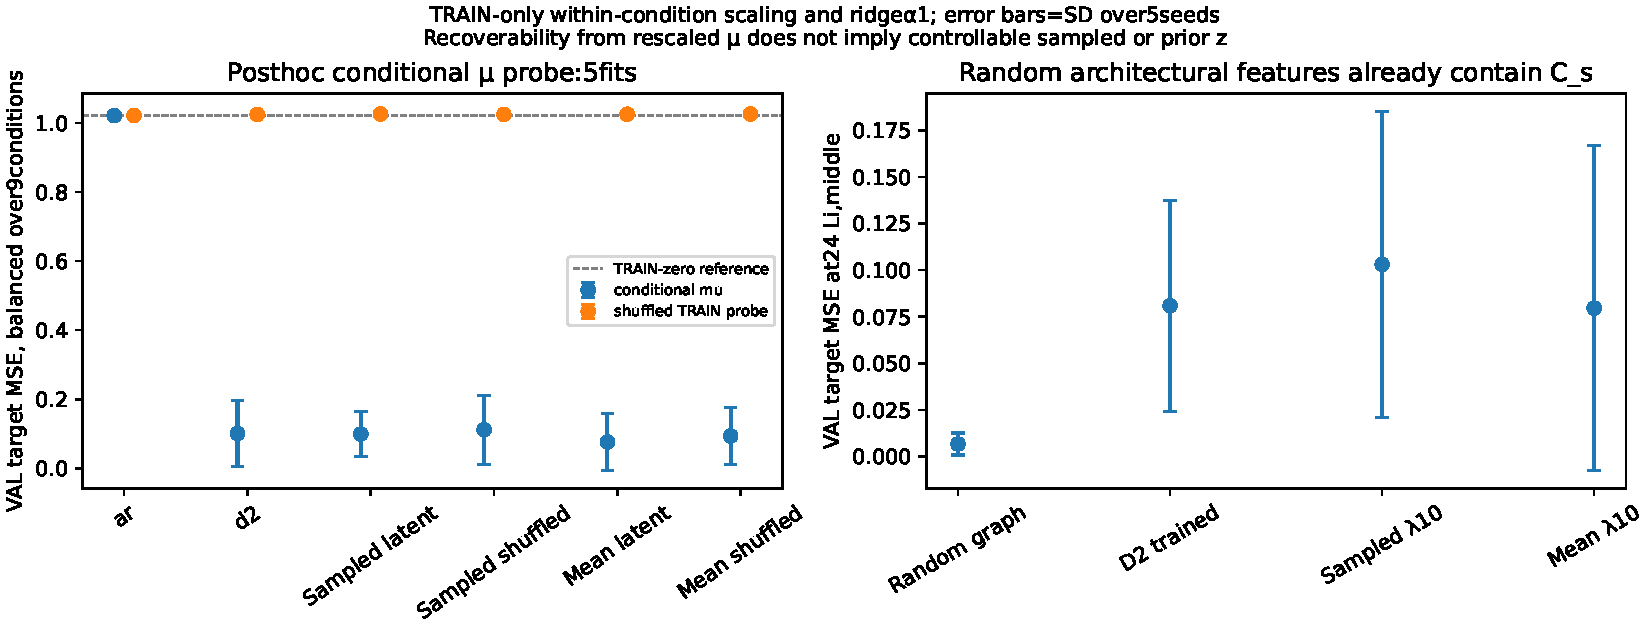
\includegraphics[width=\linewidth]{conditional_information_comparison.pdf}
\caption{Posthoc probes with TRAIN-only within-condition scaling. Left:
balanced held-out MSE over the nine cells, with five-fit SD. Right:
fixed-condition random-encoder and trained-encoder comparisons. The
nearest-shell vacancy-pair fraction, called $C_s$ in the plots, is
$C_{\rm vv}$ in the equations. These probes read deterministic means.}
\end{figure}

The scale matters. In the predeclared first-fit illustration with 986 VAL
records at fixed count and energy bin, SD$(\mu_1)$ is approximately
$1.29\times10^{-6}$ for ordinary $D=2$, $1.63\times10^{-7}$ for sampled-head
supervision, and $2.45\times10^{-8}$ for mean supervision. Posterior standard
deviations are about 0.94--0.96 and the prior standard deviation is one.
A rescaled scatter can reveal ordering in $\mu$, while adding unit-scale
Gaussian noise almost completely hides that ordering from sampled $z$.
For illustration, two equal-unit-variance Gaussians whose means differ by
$10^{-6}$ have KL $\tfrac12(10^{-6})^2=5\times10^{-13}$ nats. This example
explains the scale; it is not a substitute for the measured posteriors.

\begin{figure}[p]
\centering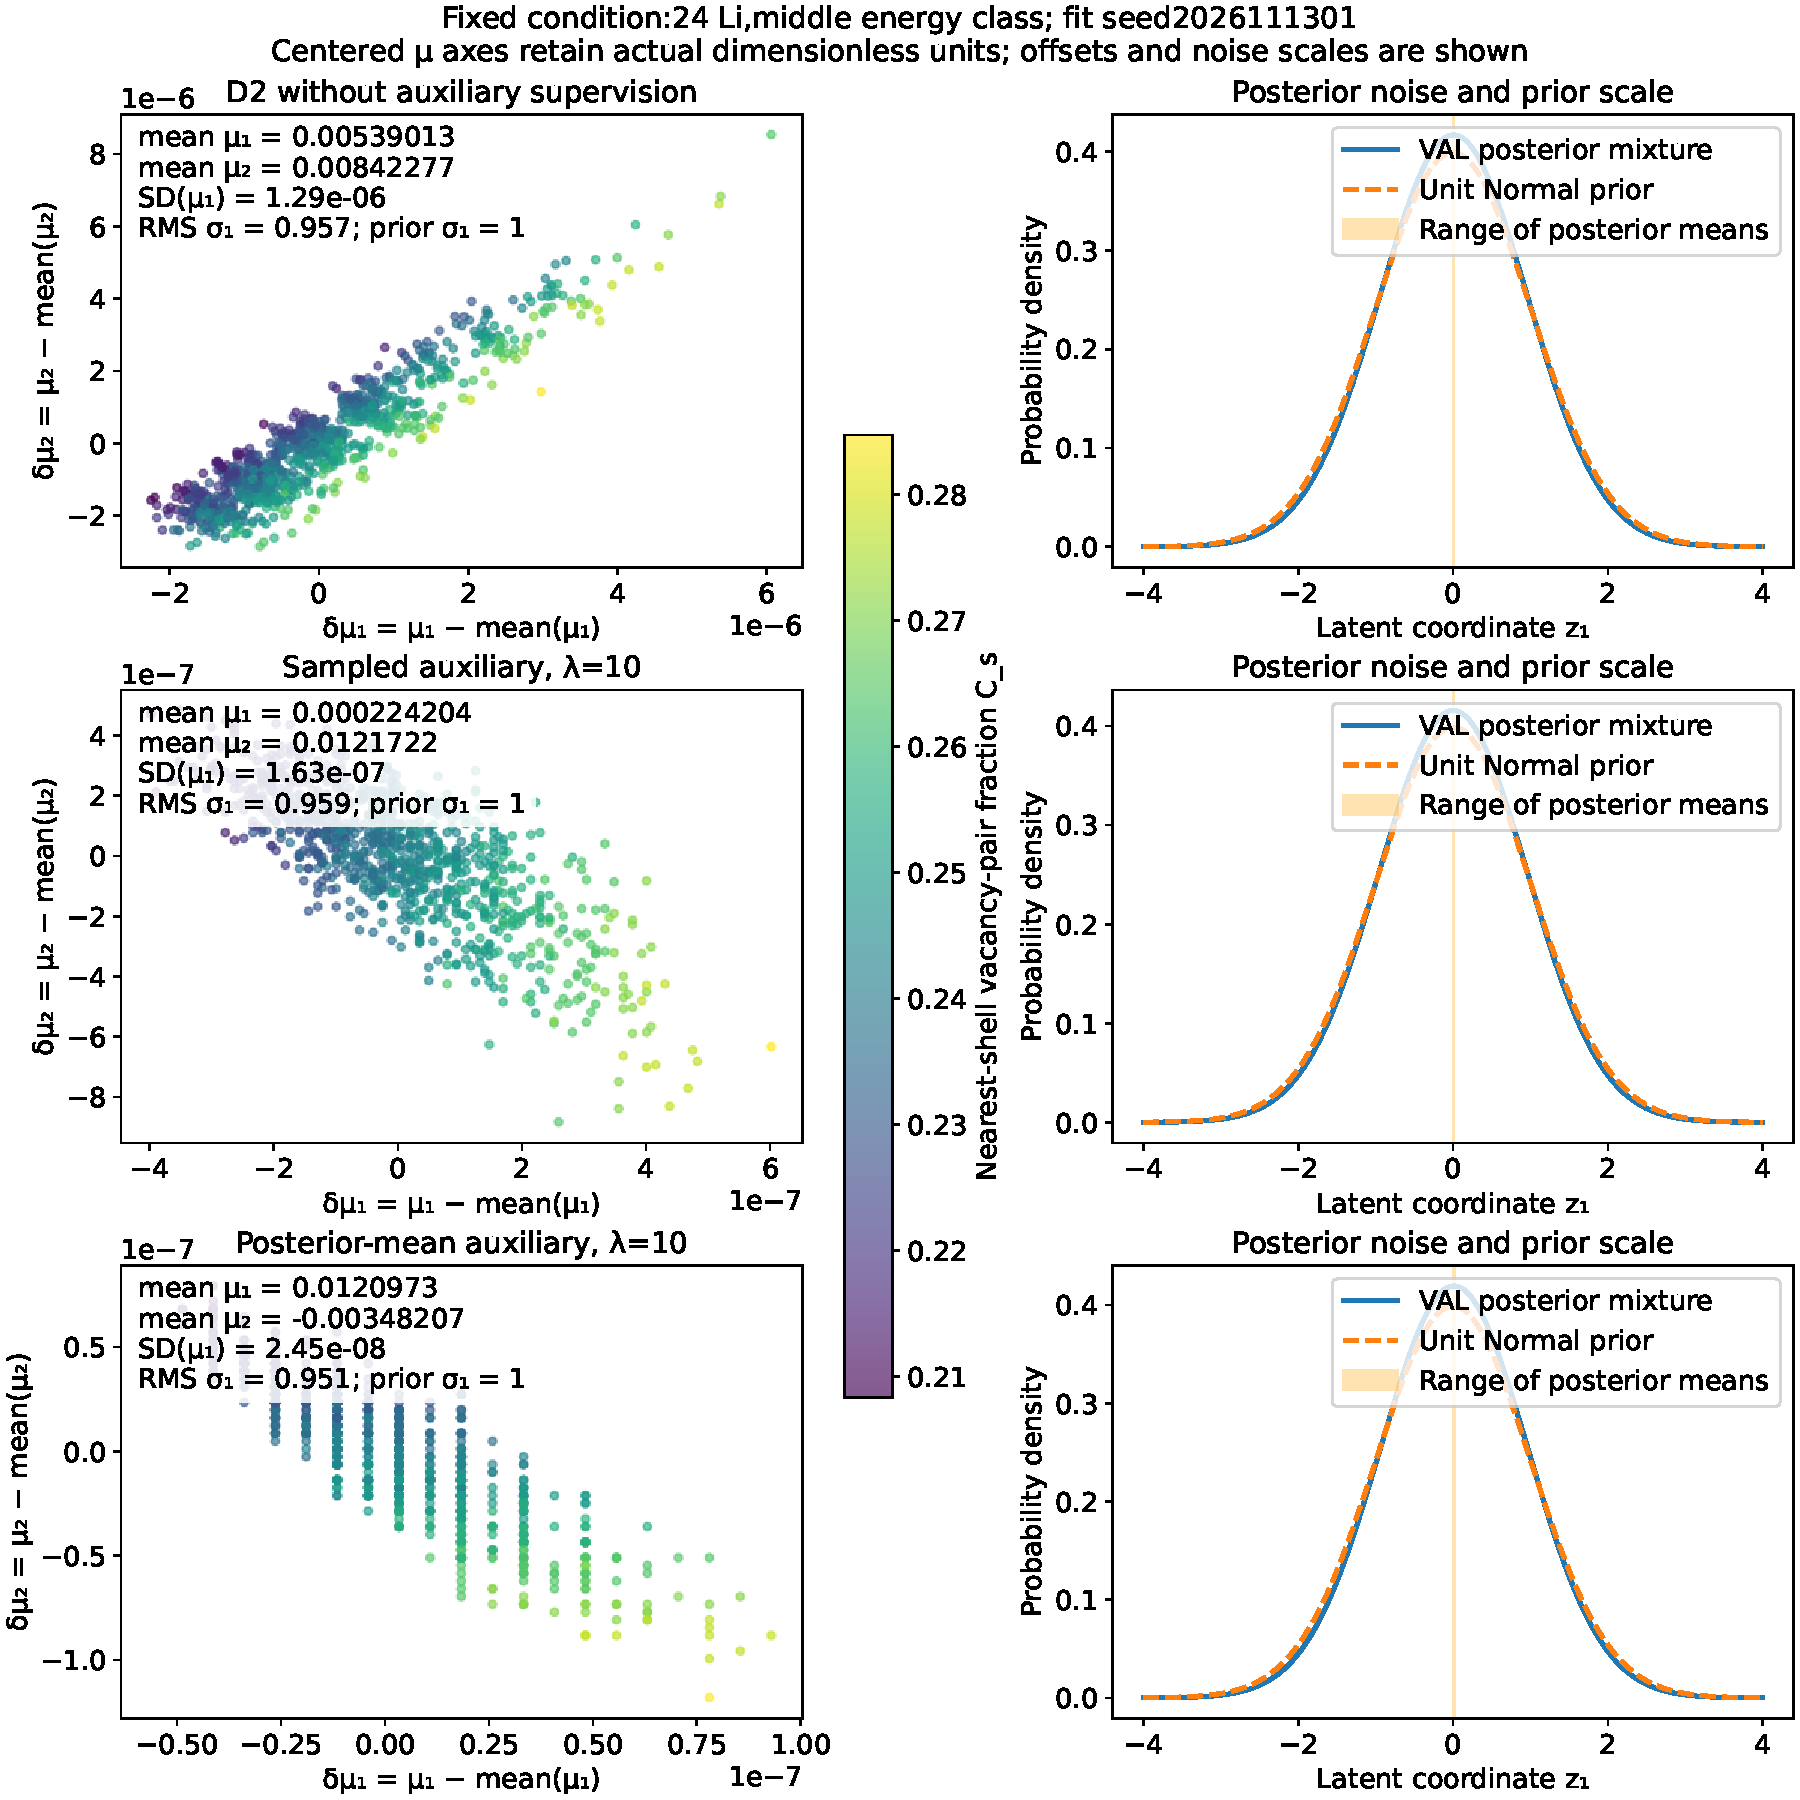
\includegraphics[width=\linewidth,height=0.85\textheight,keepaspectratio]{fixed_condition_latent_centered.pdf}
\caption{One predeclared fit and condition: $n=24$, MIDDLE, seed 2026111301.
Centered mean coordinates reveal the tiny structure-dependent variation;
the accompanying posterior-mixture panels show it relative to sampling
noise. Encoder outputs here are CPU FP32 reevaluations; moment statistics
use float64. The primary generation retains its GPU protocol. This illustration is not a selected
best fit, and its colored means do not establish prior-generation control.}
\end{figure}

We can quantify this distinction without estimating mutual information from
a scatter. Let $q_i$ be the diagonal Gaussian encoder posterior of VAL mask
$i$ in this fixed cell, and $\bar q=N^{-1}\sum_jq_j$. Take the uniform
empirical distribution over the $N=986$ VAL records. Then
\begin{equation}
I_{\rm VAL}(X;Z\mid c)=\frac1N\sum_i\KL(q_i\|\bar q)
\;\leq\;\frac1{N^2}\sum_{i,j}\KL(q_i\|q_j).
\end{equation}
The inequality follows from convexity of $-\log$:
$-\log[N^{-1}\sum_jq_j(z)]\leq N^{-1}\sum_j[-\log q_j(z)]$.
Integrating under each $q_i$ and averaging gives the right-hand side.
Pairwise Gaussian KL is analytic. A cancellation-resistant
float64 calculation, checked with an independent Gaussian implementation,
80-digit spot calculations, and a Taylor upper envelope, gives:

\begin{table}[htbp]
\centering\small
\caption{Information diagnostics for the fixed empirical VAL cell and first
fit only. The pairwise quantity is a computed upper bound, reported by order
of magnitude rather than as interval-certified last digits.}
\begin{tabular}{lrr}\toprule
Encoder & Mean KL to prior (nats) & Pairwise information bound (nats)\\\midrule
Ordinary $D=2$ & $4.06\times10^{-3}$ & $\sim7.1\times10^{-12}$\\
Sampled-head $\lambda=10$ & $3.48\times10^{-3}$ & $\sim4.2\times10^{-13}$\\
Mean-head $\lambda=10$ & $6.56\times10^{-3}$ & $\sim4.8\times10^{-15}$\\\bottomrule
\end{tabular}
\end{table}

Most KL to the prior in this illustration describes a common mismatch of
the conditional posterior mixture, rather than information distinguishing
the masks. This is a statement about the empirical encoder joint
$(X,Z)$ in one cell. It does not prove that the decoder ignores prior $z$;
the prior interventions and generated-property measurements test that
separate question. Together, they explain how informative deterministic
means can coexist with ineffective sampled-latent physical control.

The conditional probes and numerical checks introduce no new training or
oracle calls. An initial float32 moment annotation at this extremely small
scale was corrected using float64; original plots are preserved with the
precision-correction receipt. The figures here use the corrected values.

